\chapter*{Anexo 1: Manual de Usuario}
\markboth{\textbf{Anexo 1: Manual de Usuario}}{}
\addcontentsline{toc}{chapter}{Anexo 1: Manual de Usuario}

En este anexo se detalla el proceso de instalación, configuración y uso de la aplicación desarrollada.

\section*{Requisitos previos}
\addcontentsline{toc}{section}{1. Requisitos previos}

Para la ejecución del proyecto, es necesario el uso del sistema operativo Ubuntu o compatibles. Puede descargarse desde \url{https://ubuntu.com/download/desktop}, e instalarse de forma nativa (\url{https://ubuntu.com/tutorials/install-ubuntu-desktop#1-overview}) o mediante una máquina virtual utilizando herramientas como VirtualBox (\url{https://ubuntu.com/tutorials/how-to-run-ubuntu-desktop-on-a-virtual-machine-using-virtualbox#1-overview}).

Una vez instalado Ubuntu, el código fuente del proyecto puede obtenerse desde el repositorio oficial en GitHub: \url{https://github.com/juuaann03/TFG}. Para ello, se puede descargar directamente el archivo comprimido (.zip) o clonar el repositorio, utilizando el botón verde \textit{Code}.

\newpage
\section*{Configuración previa a la instalación}
\addcontentsline{toc}{section}{2. Configuración previa a la instalación}

Es necesario crear un archivo de configuración denominado \texttt{.env} en el directorio \texttt{backend}. Este archivo debe contener las claves necesarias para el funcionamiento de las APIs utilizadas:

\begin{verbatim}
	OPENROUTER_API_KEY=key1  
	RAWG_API_KEY=key2  
	JWT_SECRET_KEY=key3  
	STEAM_API_KEY=key4
\end{verbatim}

A continuación, se explica el propósito de cada clave y el procedimiento para obtenerla:

\subsection*{2.1 OPENROUTER\_API\_KEY}
\addcontentsline{toc}{subsection}{2.1 OPENROUTER\_API\_KEY}
Clave utilizada para acceder a los modelos de lenguaje que constituyen el motor principal del sistema. Se puede obtener creando una cuenta en la plataforma:  
\url{https://openrouter.ai/}

\begin{center}
	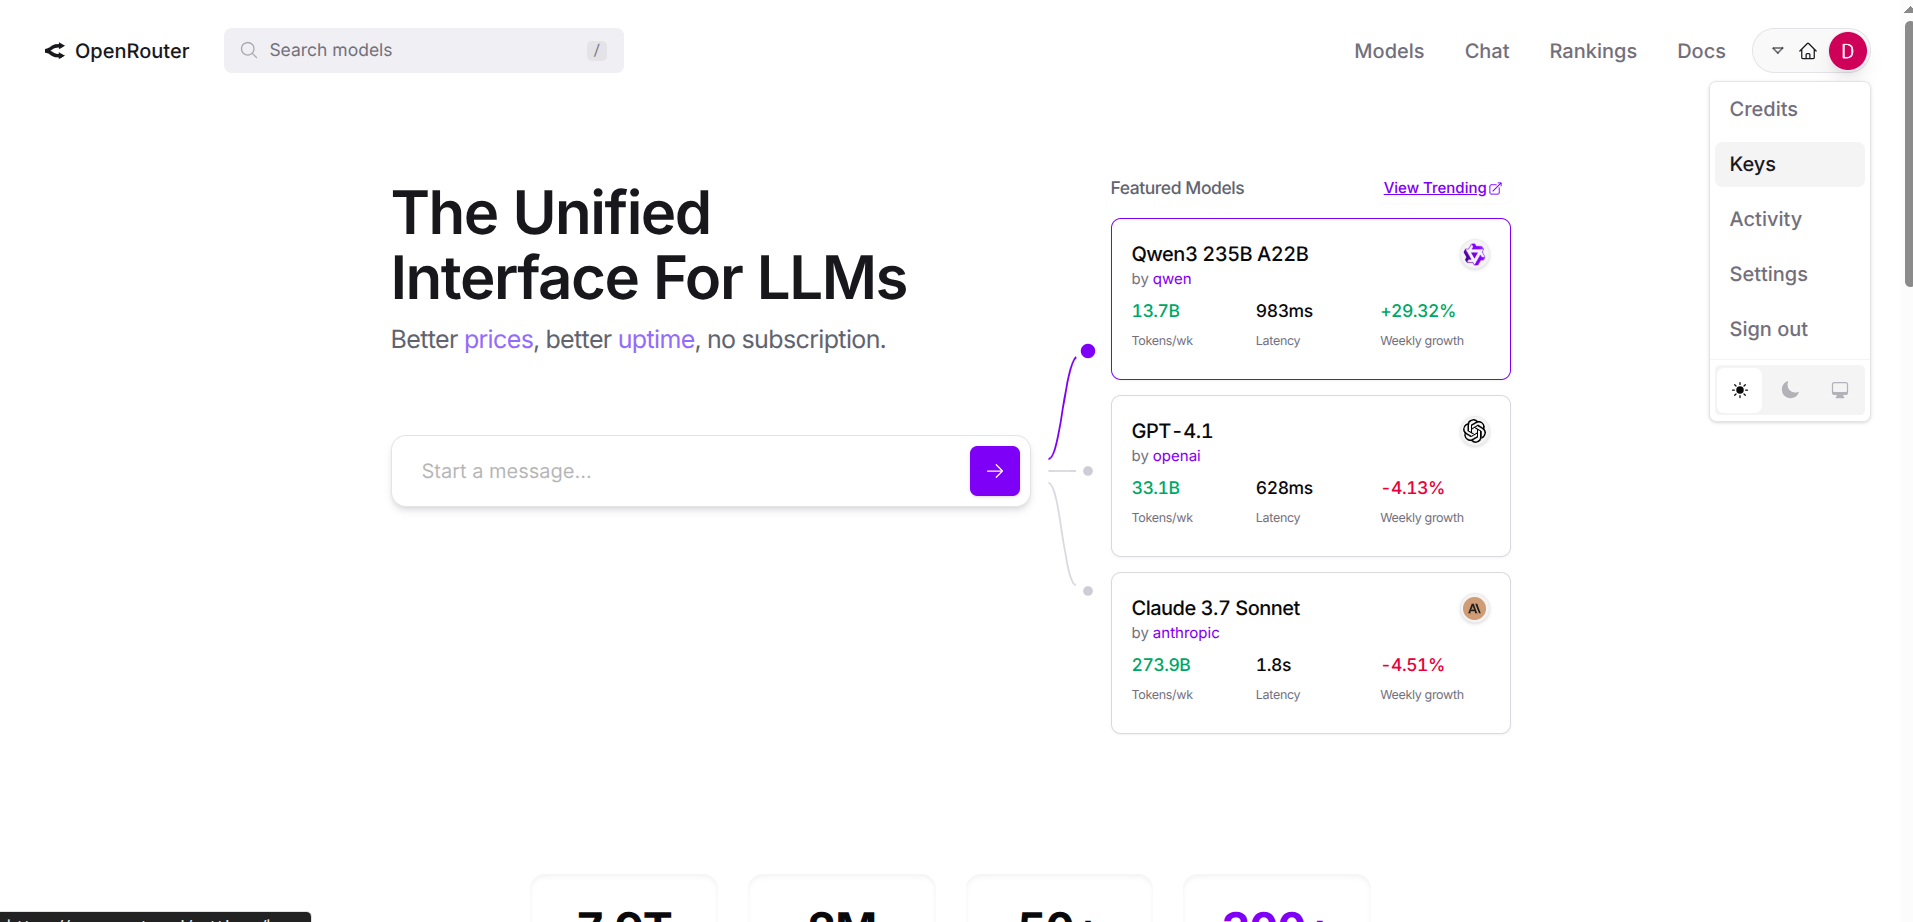
\includegraphics[width=1\textwidth]{imagenes/openRouter.png}
\end{center}

\subsection*{2.2 RAWG\_API\_KEY}
\addcontentsline{toc}{subsection}{2.2 RAWG\_API\_KEY}
Clave necesaria para acceder a datos e imágenes de videojuegos. Se obtiene tras registrarse como desarrollador en:  
\url{https://rawg.io/login?forward=developer}

\begin{center}
	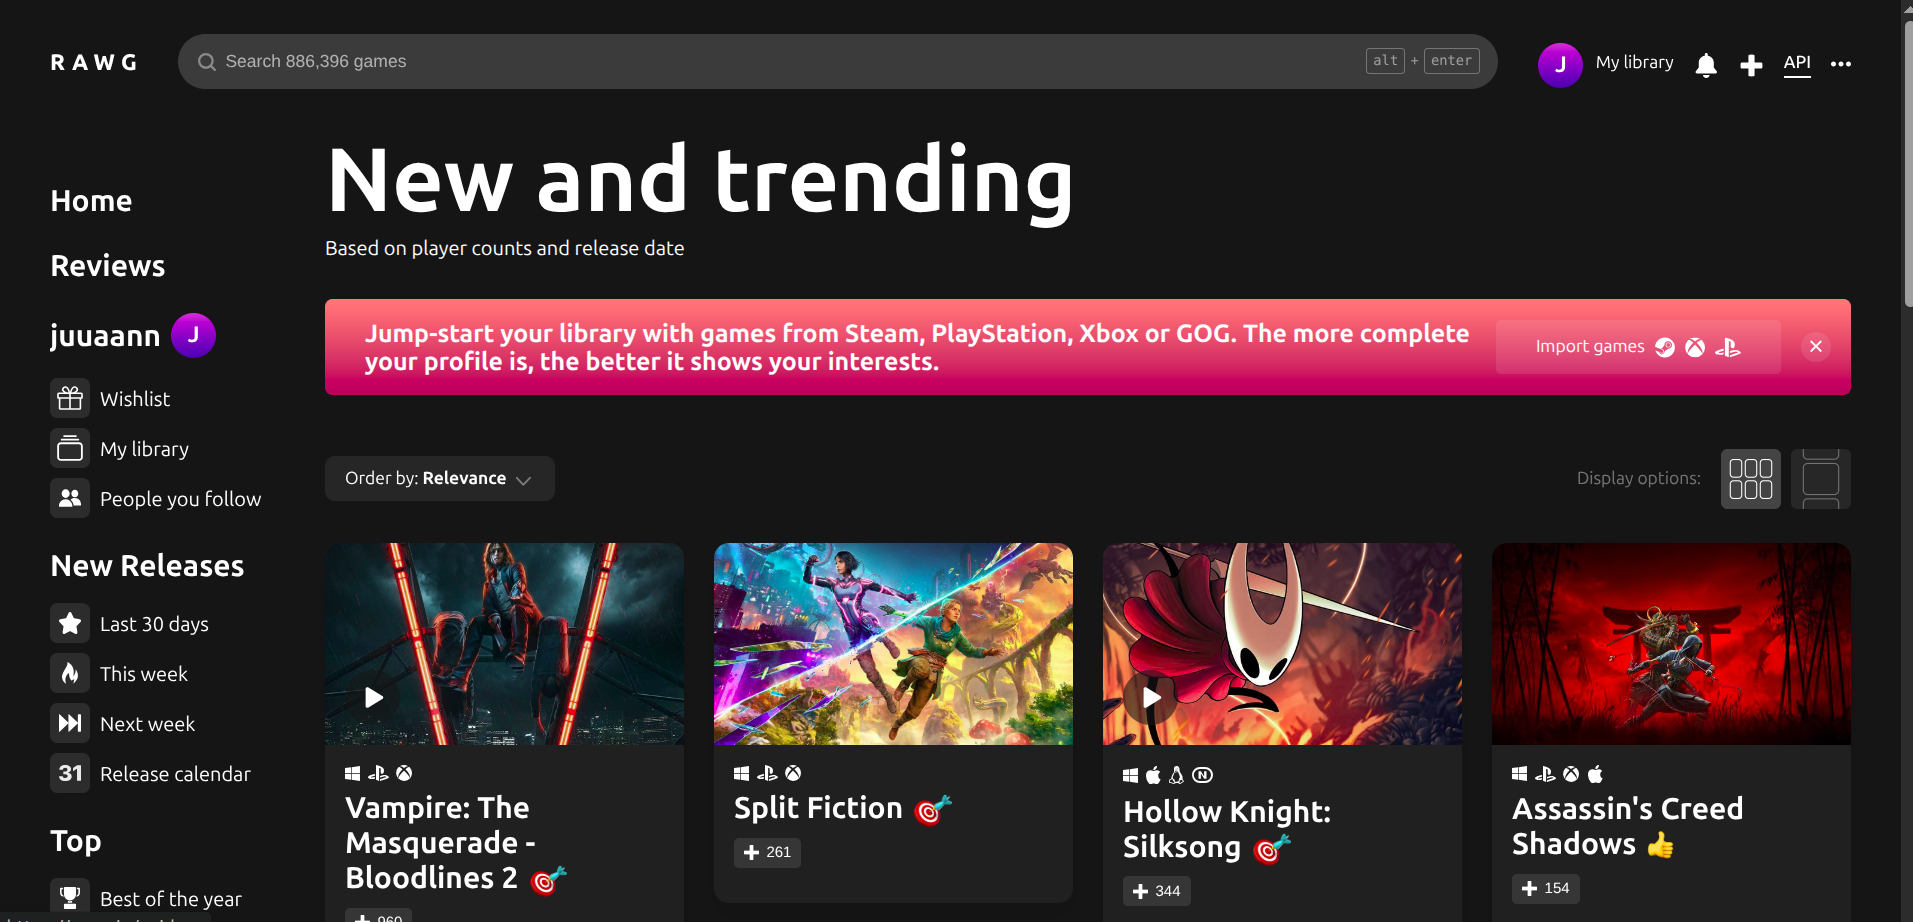
\includegraphics[width=1\textwidth]{imagenes/rawg.png}
\end{center}

\subsection*{2.3 JWT\_SECRET\_KEY}
\addcontentsline{toc}{subsection}{2.3 JWT\_SECRET\_KEY}
Clave secreta utilizada para la generación y verificación de tokens JWT (JSON Web Tokens), fundamentales en el sistema de autenticación del proyecto. Debe generarse de forma segura por el usuario mediante uno de los siguientes métodos:

\textbf{Usando Python:}
\begin{verbatim}
	import secrets
	print(secrets.token_hex(32))
\end{verbatim}

\textbf{Usando OpenSSL en la terminal:}
\begin{verbatim}
	openssl rand -hex 32
\end{verbatim}

\subsection*{2.4 STEAM\_API\_KEY}
\addcontentsline{toc}{subsection}{2.4 STEAM\_API\_KEY}
Clave requerida para acceder a la API de Steam. Es necesario tener una cuenta con al menos 5 dólares invertidos para poder generarla en:  
\url{https://steamcommunity.com/dev/apikey}

\newpage

\section*{Proceso de instalación}
\addcontentsline{toc}{section}{3. Proceso de instalación}

Desde una terminal ubicada en la raíz del proyecto, ejecutar el siguiente comando:

\begin{verbatim}
	./instalador.sh
\end{verbatim}

En caso de no disponer de permisos de ejecución:

\begin{verbatim}
	chmod +x ./instalador.sh
\end{verbatim}

Este script automatiza la instalación de todos los componentes: base de datos, backend y frontend. Durante el proceso pueden aparecer preguntas relacionadas con la configuración de Angular; se recomienda aceptar todas las opciones por defecto (presionar \texttt{Enter}).

Si es necesario reinstalar un componente de forma individual, puede ejecutarse su instalador correspondiente desde su carpeta específica.

Al finalizar la instalación, los servicios se ejecutarán automáticamente en segundo plano. Las salidas del backend y del frontend se almacenan en archivos \texttt{log} ubicados en la raíz del proyecto.

\subsection*{3.1 Parar los servicios}
\addcontentsline{toc}{subsection}{3.1 Parar los servicios}
Para detener todos los procesos que se encuentran en ejecución:

\begin{verbatim}
	./detener.sh
\end{verbatim}

\subsection*{3.2 Reiniciar la aplicación}
\addcontentsline{toc}{subsection}{3.2 Reiniciar la aplicación}

Para volver a iniciar todos los servicios del proyecto:

\begin{verbatim}
	./inicializarProyecto.sh
\end{verbatim}

\noindent La interfaz web estará disponible en: \url{http://localhost:4200/}

\newpage
\section*{Uso de la aplicación}
\addcontentsline{toc}{section}{4. Uso de la aplicación}

En la página principal, el usuario puede realizar peticiones simples ingresándolas en el campo de texto y pulsando \textit{Enter} o el botón de envío. También es posible registrarse o iniciar sesión a través de los botones correspondientes, introduciendo sus credenciales.

Una vez autenticado, el usuario tiene acceso a funcionalidades personalizadas. En la pantalla principal se muestran:

\begin{itemize}
	\item Últimos lanzamientos adaptados a sus gustos.
	\item Las seis recomendaciones más recientes.
	\item Un campo para realizar consultas que generan recomendaciones personalizadas. Estas pueden influir en la actualización de su perfil (por ejemplo, si el usuario indica que ha comprado una consola determinada).
\end{itemize}

Desde el menú de ajustes de cuenta, se puede:

\begin{itemize}
	\item Visualizar la información actual sobre preferencias de videojuegos.
	\item Eliminar la cuenta o cambiar la contraseña.
	\item Borrar toda la información relacionada con videojuegos.
	\item Vincular una cuenta de Steam mediante la introducción del \texttt{SteamID64}, el cual se puede consultar en: \url{https://help.steampowered.com/es/faqs/view/2816-BE67-5B69-0FEC}
\end{itemize}

Adicionalmente, existe un campo de entrada para modificar manualmente la información del usuario, permitiendo registrar eventos como la venta de una consola, la aparición de una necesidad especial, cambios de idioma, entre otros.
